%! TEX program = xelatex
% Please make sure you insert your
% data according to the instructions in PoSauthmanual.pdf
\documentclass[a4paper,11pt]{article}
\usepackage{pos}

\title{HMC with Normalizing Flows}
%% \ShortTitle{Short Title for header}

\author*[a]{Sam Foreman}
\author[b, c]{Taku Izubuchi}
\author[d]{Luchang Jin}
\author[a]{Xiao-Yong Jin}
\author[a]{James C. Osborn}
\author[b]{Akio Tomiya}

\affiliation[a]{Argonne National Laboratory,\\
  Lemont, IL 60439}

\affiliation[b]{RIKEN,\\
 2-1 Hirosawa, Wako, Saitama, 351-0198, Japan}

\affiliation[c]{Brookhaven National Laboratory,\\
 Upton, NY 11973}

\affiliation[d]{Dept. of Physics, University of Connecticut,\\
 Storrs, CT 06269}

\emailAdd{foremans@anl.gov}
\emailAdd{izubuchi@bnl.gov}
\emailAdd{luchang.jin@uconn.edu}
\emailAdd{xjin@anl.gov}
\emailAdd{osborn@alcf.anl.gov}

\abstract{%
    We propose using Normalizing Flows as a trainable kernel within the
    molecular dynamics update of Hamiltonian Monte Carlo (HMC).
    %
    By learning (invertible) transformations that simplify our dynamics, we can
    outperform traditional methods at generating independent configurations.
    %
    We show that, using a carefully constructed network architecture, our
    approach can be easily scaled to large lattice volumes with minimal
    retraining effort.
}

\FullConference{%
  % *** FIXME: Name of conference, ***\\
  The 38th International Symposium on Lattice Field Theory\\
  % *** FIXME: day-day Month YEAR ***\\
  26-30 July 2021\\
  % *** FIXME: Location, City, Country ***
  Zoom / Gather @ MIT, Cambridge MA, USA\\
}

%% \tableofcontents

\begin{document}
\maketitle


\section{Introduction}
For a random variable \(z\) with a given distribution \(z \sim r(z)\), and an
invertible function \(x = f(z)\) with \(z = f^{-1}(x)\), we can use the change
of variables formula to write
%
\begin{equation}
    p(x) = r(z)\left|\det\frac{\partial z}{\partial x}\right| =
    r(f^{-1}(x))\left|\det\frac{\partial f^{-1}}{\partial x}\right|
\end{equation}
%
where \(r(z)\) is the (simple) prior density, and our goal is to generate
independent samples from the (difficult) target distribution \(p(x)\).
%
This can be done using \emph{normalizing flows} to construct a model density
\(q(x)\) that approximates the target distribution, i.e. \(q(\cdot)\simeq
p(\cdot)\) for a suitably-chosen flow \(f\).

\begin{figure}[htpb]
    \centering
    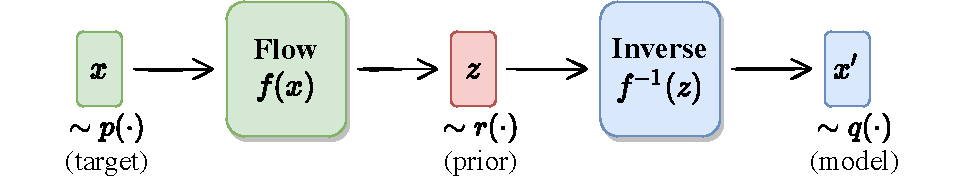
\includegraphics[width=0.9\textwidth]{assets/flow_model.pdf}
    \caption{\label{fig:flow_model} Using a flow to generate data \(x'\). Image adapted from~\cite{}}  % TODO: Fill in citations
\end{figure}

\begin{thebibliography}{99}
\bibitem{...}
....

\end{thebibliography}

\end{document}
